\chapter{Architecture}\label{Chap:Architecture}
\begin{figure}[!htb]
   \centering
   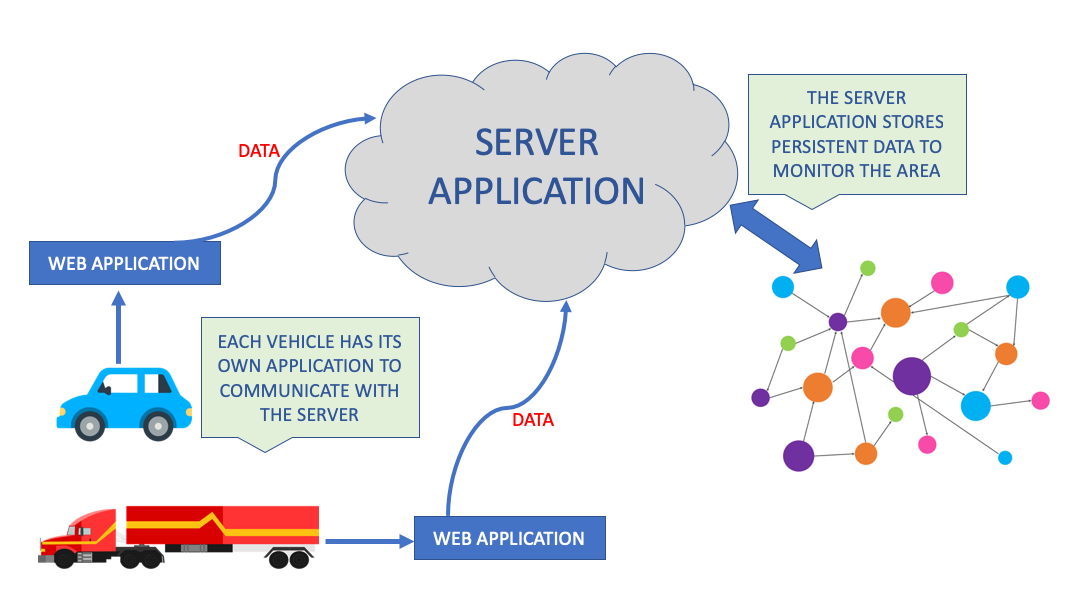
\includegraphics[width=\textwidth]{architecture.png}
   \caption{Architecture of the system.}\label{Fig:ArchNoImpl}
\end{figure}
The system consists of three principal components:
\begin{itemize}
  \item Server: this component is responsible for the validation of data, supervision of the system and interaction with the database
    to store persistent data;
  \item Client: this component consist of an application, located on the vehicle, that communicates with the server and provide it with information about the vehicle (e.g. position, entry and exit time);
  \item Database: where are stored data about the current state of the area, i.e. actual capacity of places, position of vehicles and
  average times spent in each place.
\end{itemize}
